\documentclass[12pt,a4paper]{article}

% ── Codificación y idioma ────────────────────────────────────────────────────
\usepackage{fontspec}
\usepackage{polyglossia}
\setmainlanguage{spanish}
\usepackage{lmodern}

% ── Márgenes y geometría ─────────────────────────────────────────────────────
\usepackage[top=2.5cm, bottom=2.5cm, left=3cm, right=3cm]{geometry}

% ── Gráficos y figuras ───────────────────────────────────────────────────────
\usepackage{graphicx}
\usepackage{float}
\usepackage{caption}
\usepackage{subcaption}
\graphicspath{{../data/output/}}

% ── Tablas ───────────────────────────────────────────────────────────────────
\usepackage{booktabs}
\usepackage{array}
\usepackage{multirow}
\usepackage{xcolor}
\usepackage{colortbl}

% ── Matemáticas ──────────────────────────────────────────────────────────────
\usepackage{amsmath}
\usepackage{amssymb}

% ── Código ───────────────────────────────────────────────────────────────────
\usepackage{listings}
\lstset{
  basicstyle=\ttfamily\footnotesize,
  backgroundcolor=\color{gray!10},
  frame=single,
  breaklines=true,
  language=Python,
  keywordstyle=\color{blue},
  commentstyle=\color{gray},
}

% ── Hipervínculos ────────────────────────────────────────────────────────────
\usepackage{hyperref}
\hypersetup{
  colorlinks=true,
  linkcolor=blue!60!black,
  urlcolor=blue!60!black,
  citecolor=blue!60!black,
}

% ── Cabecera y pie de página ─────────────────────────────────────────────────
\usepackage{fancyhdr}
\pagestyle{fancy}
\fancyhf{}
\rhead{BRP Bicing Barcelona}
\lhead{MD009 -- Eines avançades d'anàlisi}
\rfoot{\thepage}

% ── Colores para tablas ──────────────────────────────────────────────────────
\definecolor{bestgreen}{RGB}{212,237,218}
\definecolor{headerblue}{RGB}{70,130,180}
\definecolor{lightgray}{gray}{0.93}

% ─────────────────────────────────────────────────────────────────────────────
\title{
  \vspace{-1cm}
  {\Large Optimización de Rutas de Redistribución (BRP)} \\[6pt]
  {\large Bicing Barcelona --- Predicción de Demanda y Planificación de Flota} \\[4pt]
  {\normalsize MD009 -- Eines avançades d'anàlisi}
}
\author{Ferran Tubert}
\date{Abril 2026}

\begin{document}

\maketitle
\thispagestyle{fancy}
\tableofcontents
\newpage

% =============================================================================
\section{Introducción}
% =============================================================================

El sistema de bicicletas públicas Bicing de Barcelona gestiona más de 548 estaciones
distribuidas por la ciudad. Uno de los principales retos operativos es el
\textbf{desequilibrio de ocupación}: algunas estaciones se quedan vacías mientras otras
se saturan, especialmente en las horas punta de la mañana y la tarde.

El \textbf{Bike Redistribution Problem (BRP)} consiste en planificar las rutas de una
flota de camiones para mover bicicletas de estaciones con superávit a estaciones con
déficit, minimizando el desequilibrio global con los recursos disponibles.

Este informe documenta el pipeline completo:
\begin{enumerate}
  \item Análisis exploratorio de los datos de telemetría (EDA).
  \item Entrenamiento de dos modelos predictivos: XGBoost y GRU (LSTM simplificado).
  \item Evaluación y selección del mejor modelo.
  \item Integración del modelo en el algoritmo BRP para planificación proactiva de rutas.
\end{enumerate}

\paragraph{Datos.}
Telemetría horaria de Bicing, octubre 2023 -- septiembre 2025 ($\sim$8,9 millones de
registros, 548 estaciones). Los datos incluyen disponibilidad de bicicletas,
capacidad, altitud, coordenadas geográficas y variables temporales.

% =============================================================================
\section{Estructura del Código}
% =============================================================================

El proyecto sigue una estructura modular con cuatro notebooks independientes:

\begin{center}
\begin{tabular}{lll}
\toprule
\textbf{Notebook} & \textbf{Función} & \textbf{Output principal} \\
\midrule
\texttt{EDA.ipynb}     & Análisis exploratorio y feature engineering & \texttt{bicing\_full.parquet} \\
\texttt{XGBoost.ipynb} & Entrenamiento y evaluación XGBoost          & \texttt{xgboost\_bicing.ubj} \\
\texttt{LSTM.ipynb}    & Entrenamiento y evaluación GRU              & \texttt{lstm\_bicing.keras}  \\
\texttt{BRP.ipynb}     & Optimización de rutas con el mejor modelo   & Rutas + métricas \\
\bottomrule
\end{tabular}
\end{center}

\subsection{Pipeline de datos}

El flujo de datos sigue la siguiente cadena:

\begin{enumerate}
  \item \textbf{EDA}: carga de datos crudos, limpieza, ingeniería de features
        (lags, codificación cíclica, media de análogos), split temporal y
        exportación de \texttt{bicing\_full.parquet} y \texttt{bicing\_model\_ready.parquet}.
  \item \textbf{XGBoost / GRU}: leen el parquet correspondiente, dividen en
        \textit{train} (oct.\ 2023 -- may.\ 2025), \textit{val} (jun.--jul.\ 2025)
        y \textit{test} (ago.--sep.\ 2025), entrenan con early stopping y guardan
        el modelo serializado en \texttt{models/}.
  \item \textbf{BRP}: carga ambos modelos, compara métricas sobre el test, selecciona
        el mejor y genera predicciones para el escenario de redistribución.
\end{enumerate}

\subsection{Split temporal}

\begin{center}
\begin{tabular}{llcc}
\toprule
\textbf{Conjunto} & \textbf{Período} & \textbf{Filas} & \textbf{Proporción} \\
\midrule
Train & Oct 2023 -- May 2025 & 7.260.104 & 82,3\,\% \\
Val   & Jun 2025 -- Jul 2025 &   774.850 &  8,8\,\% \\
Test  & Ago 2025 -- Sep 2025 &   781.327 &  8,9\,\% \\
\bottomrule
\end{tabular}
\end{center}

El corte temporal estricto garantiza que los modelos nunca ven datos futuros durante
el entrenamiento (sin \textit{data leakage}).

% =============================================================================
\section{Modelos}
% =============================================================================

\subsection{Baseline de persistencia}

El modelo de referencia predice que el estado en $t$ será idéntico al de $t-1\,\text{h}$:
\[
  \hat{y}_t = \frac{\text{bikes\_lag\_1h}_t}{\text{capacity}}
\]
Este baseline ya obtiene un $R^2$ elevado ($\approx 0{,}862$) por la fuerte inercia horaria
del sistema.

\subsection{XGBoost}

\paragraph{Features seleccionadas.}
\begin{itemize}
  \item \textbf{Lags temporales}: \texttt{bikes\_lag\_1h}, \texttt{bikes\_lag\_24h},
        \texttt{bikes\_lag\_168h} (inercia horaria, ciclo diario y semanal).
  \item \textbf{Contexto histórico}: \texttt{bikes\_analog\_mean} (media de semanas
        análogas; Peláez-Rodríguez et al., 2024).
  \item \textbf{Estáticas de estación}: \texttt{capacity}, \texttt{altitude}.
  \item \textbf{Temporales}: \texttt{hour}, \texttt{day\_of\_week}, \texttt{month}.
\end{itemize}

\paragraph{Hiperparámetros (búsqueda Optuna, 50 trials).}
\begin{center}
\begin{tabular}{ll}
\toprule
\textbf{Parámetro} & \textbf{Valor} \\
\midrule
\texttt{n\_estimators}    & 883 (early stopping) \\
\texttt{learning\_rate}   & 0,156 \\
\texttt{max\_depth}       & 8 \\
\texttt{min\_child\_weight} & 11 \\
\texttt{subsample}        & 0,621 \\
\texttt{colsample\_bytree} & 0,770 \\
\bottomrule
\end{tabular}
\end{center}

\subsection{GRU (LSTM simplificado)}

Se implementó un modelo \textbf{GRU global multi-estación} entrenado en modo
\textit{full} (548 estaciones). Para hacerlo ejecutable en un Mac M1 sin GPU externa,
se aplicaron las siguientes optimizaciones respecto al diseño original:

\begin{center}
\begin{tabular}{lcc}
\toprule
\textbf{Parámetro} & \textbf{Original} & \textbf{Optimizado} \\
\midrule
Lookback          & 168\,h & 48\,h \\
Sequence stride   & 12     & 24    \\
Batch size        & 4.096  & 8.192 \\
Épocas v0 / final & 12 / 20 & 6 / 10 \\
Capas GRU         & 2 (64+32) & 1 (48) \\
Build. datasets   & Filtro por estación $O(n{\times}S)$ & \texttt{groupby} único $O(n)$ \\
\bottomrule
\end{tabular}
\end{center}

\paragraph{Arquitectura final.}

\begin{lstlisting}
seq_input (48 x 7) --> GRU(48) --> Dropout(0.2) --> gru_out
aux_input (6,)     -----------------------------------+
sta_input () int   --> Embedding(548, 16) ------------+
                       Concatenate --> Dense(48, relu) --> Dropout
                       --> Dense(24, relu) --> Dense(1, sigmoid)
\end{lstlisting}

El embedding de estación captura la heterogeneidad residual (altitud, perfil de uso)
que no queda completamente explicada por las features numéricas. Total de parámetros: $\approx$25.000.

% =============================================================================
\section{Resultados y Evaluación de los Modelos}
% =============================================================================

\subsection{Métricas comparativas (conjunto test, Ago--Sep 2025)}

\begin{table}[H]
\centering
\caption{Comparación de modelos sobre el conjunto de test.}
\label{tab:metricas}
\begin{tabular}{lccc}
\toprule
\textbf{Modelo} & \textbf{MAE} & \textbf{RMSE} & $\boldsymbol{R^2}$ \\
\midrule
Baseline (persistencia \texttt{lag\_1h}) & 0,06489 & 0,10200 & 0,86270 \\
GRU (LSTM simplificado)                  & 0,17656 & 0,20800 & 0,43035 \\
\rowcolor{bestgreen}
XGBoost final                            & \textbf{0,06098} & \textbf{0,09006} & \textbf{0,89297} \\
\bottomrule
\end{tabular}
\end{table}

\paragraph{Conclusión.}
El XGBoost supera al baseline en todas las métricas ($\Delta$MAE\,$= -6{,}0\,\%$,
$\Delta R^2 = +3{,}5\,\text{pp}$) y al GRU por un margen muy amplio. El GRU
simplificado (48\,h lookback, 1 capa, 6+10 épocas) no converge lo suficiente:
con $R^2 = 0{,}43$ queda por debajo incluso del baseline de persistencia. El
XGBoost es el modelo seleccionado para el BRP.

\subsection{Curvas de aprendizaje del GRU}

\begin{figure}[H]
\centering
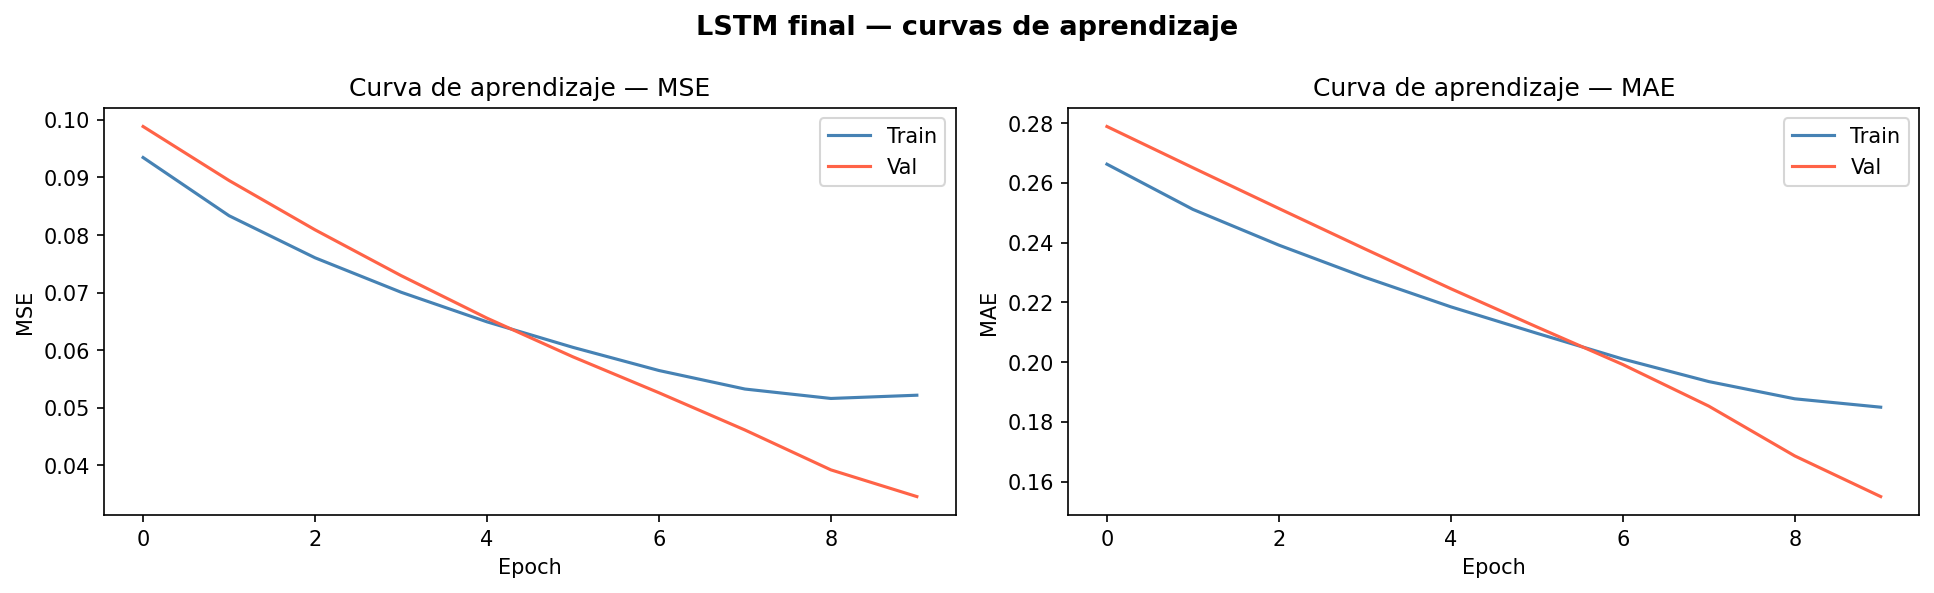
\includegraphics[width=0.85\textwidth]{LSTM_01_lstm_final__curvas_de_aprendizaje.png}
\caption{Curvas de pérdida y MAE del GRU (train vs.\ validación). La brecha entre
  train y val indica subajuste: el modelo necesita más épocas o mayor lookback para
  capturar la dinámica temporal.}
\label{fig:lstm_curves}
\end{figure}

\subsection{Análisis de residuos del GRU}

\begin{figure}[H]
\centering
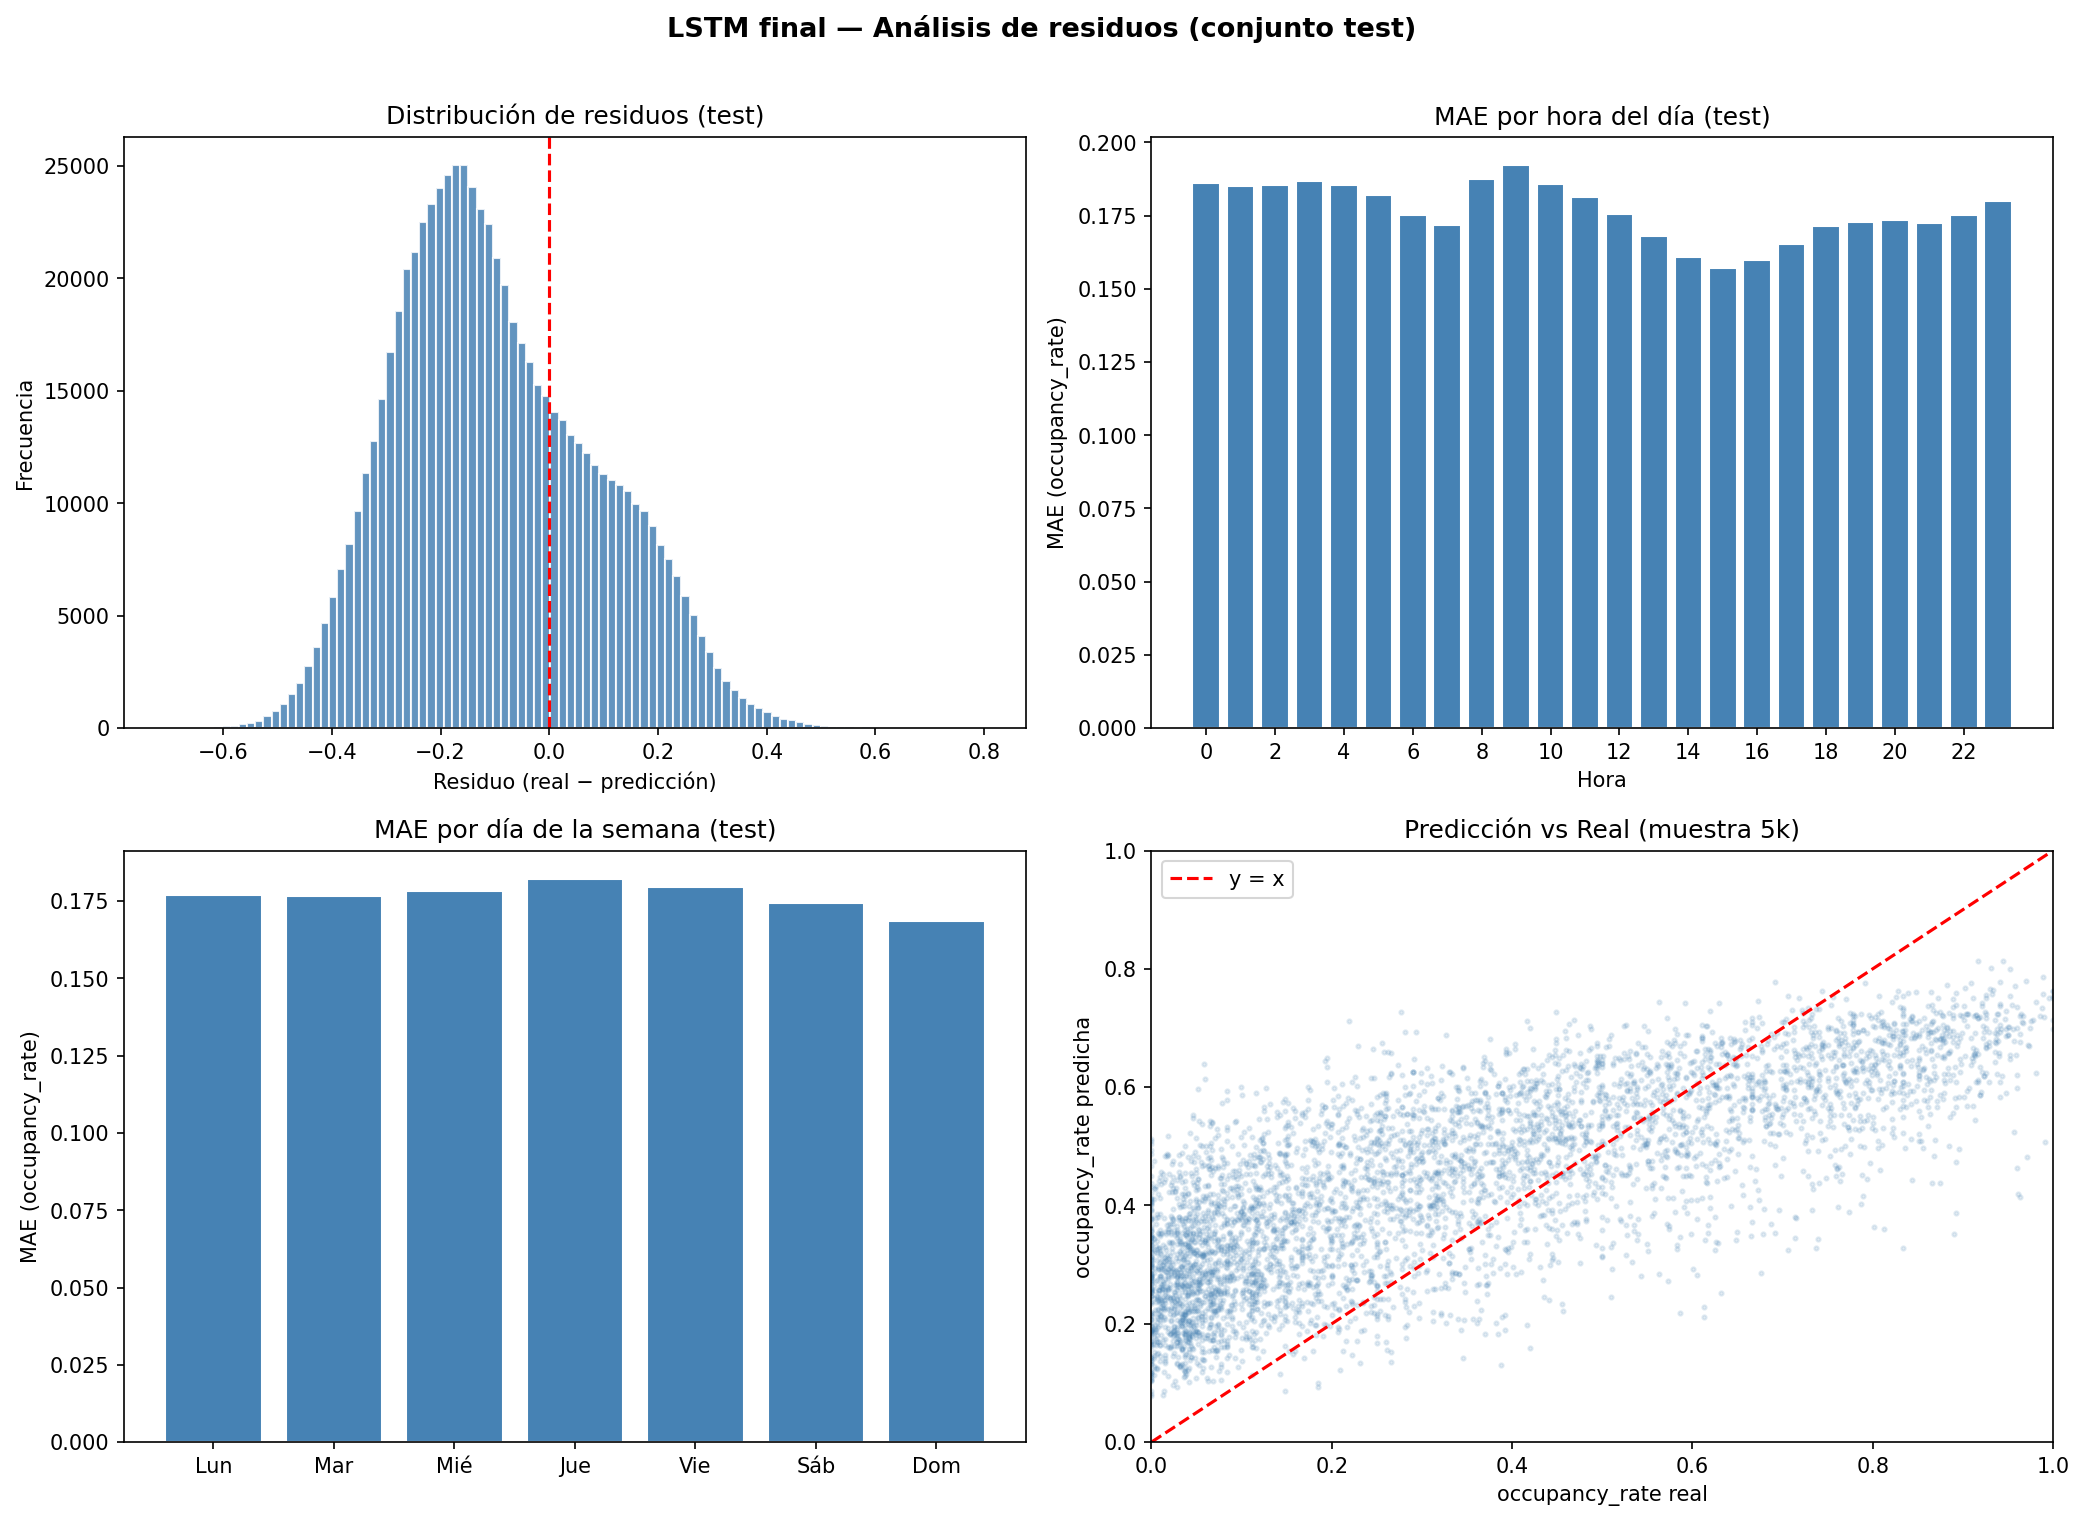
\includegraphics[width=0.85\textwidth]{LSTM_02_lstm_final__análisis_de_residuos_conjunto_test.png}
\caption{Análisis de residuos del GRU. El error medio por hora muestra el mismo patrón
  que XGBoost (máximo en franjas 7--9\,h y 17--19\,h), pero con magnitudes
  significativamente mayores.}
\label{fig:lstm_residuals}
\end{figure}

\subsection{Importancia de features en XGBoost}

La figura~\ref{fig:xgb_comparison} muestra la comparación directa entre modelos.
La contribución relativa de features en XGBoost (por \textit{gain}) está ordenada así:

\begin{enumerate}
  \item \texttt{bikes\_lag\_1h} (domina en todas las métricas; $\sim$88\,\% importancia RF).
  \item \texttt{bikes\_analog\_mean} (contexto histórico condicional; supera a lags largos).
  \item \texttt{capacity} (modulador estructural de la dinámica de llenado).
  \item \texttt{altitude} (efecto gravitacional: estaciones en cota alta acumulan bicis).
  \item \texttt{hour}, \texttt{day\_of\_week}, \texttt{month} (ciclos temporales).
\end{enumerate}

\begin{figure}[H]
\centering
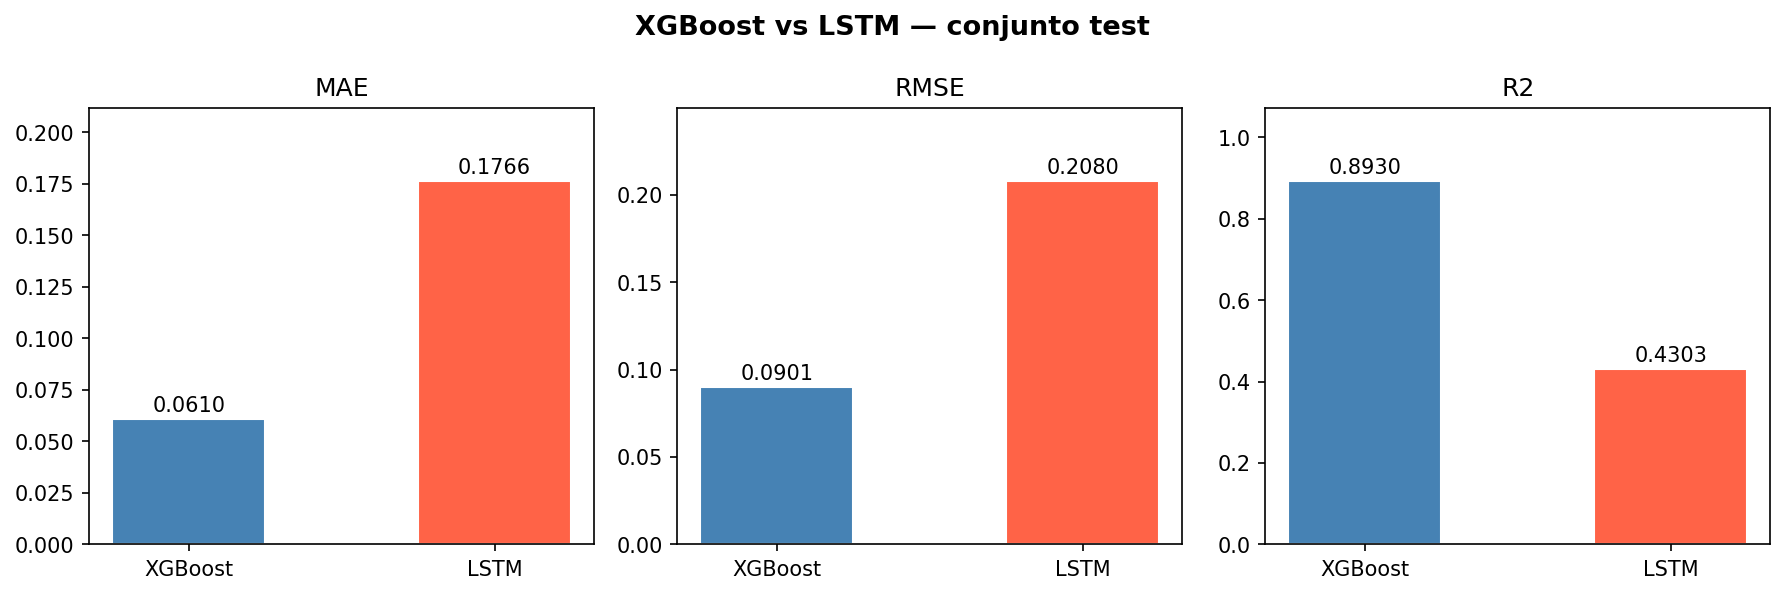
\includegraphics[width=0.85\textwidth]{LSTM_05_xgboost_vs_lstm__conjunto_test.png}
\caption{Comparación directa XGBoost vs.\ GRU en el conjunto test. El XGBoost obtiene
  un MAE $\approx 3\times$ menor y un $R^2$ $\approx 2\times$ mayor.}
\label{fig:xgb_comparison}
\end{figure}

\subsection{Error por hora del día (XGBoost)}

El MAE es máximo en las franjas de cambio de tendencia (7--9\,h y 17--19\,h) y mínimo
en horas nocturnas (1--5\,h). El error medio en test equivale a \textbf{1,66 bicicletas
por estación}, lo que es suficiente para priorizar intervenciones de redistribución con
un margen operativo razonable.

% =============================================================================
\section{Análisis Exploratorio (EDA)}
% =============================================================================

\subsection{Desequilibrio de ocupación}

\begin{figure}[H]
\centering
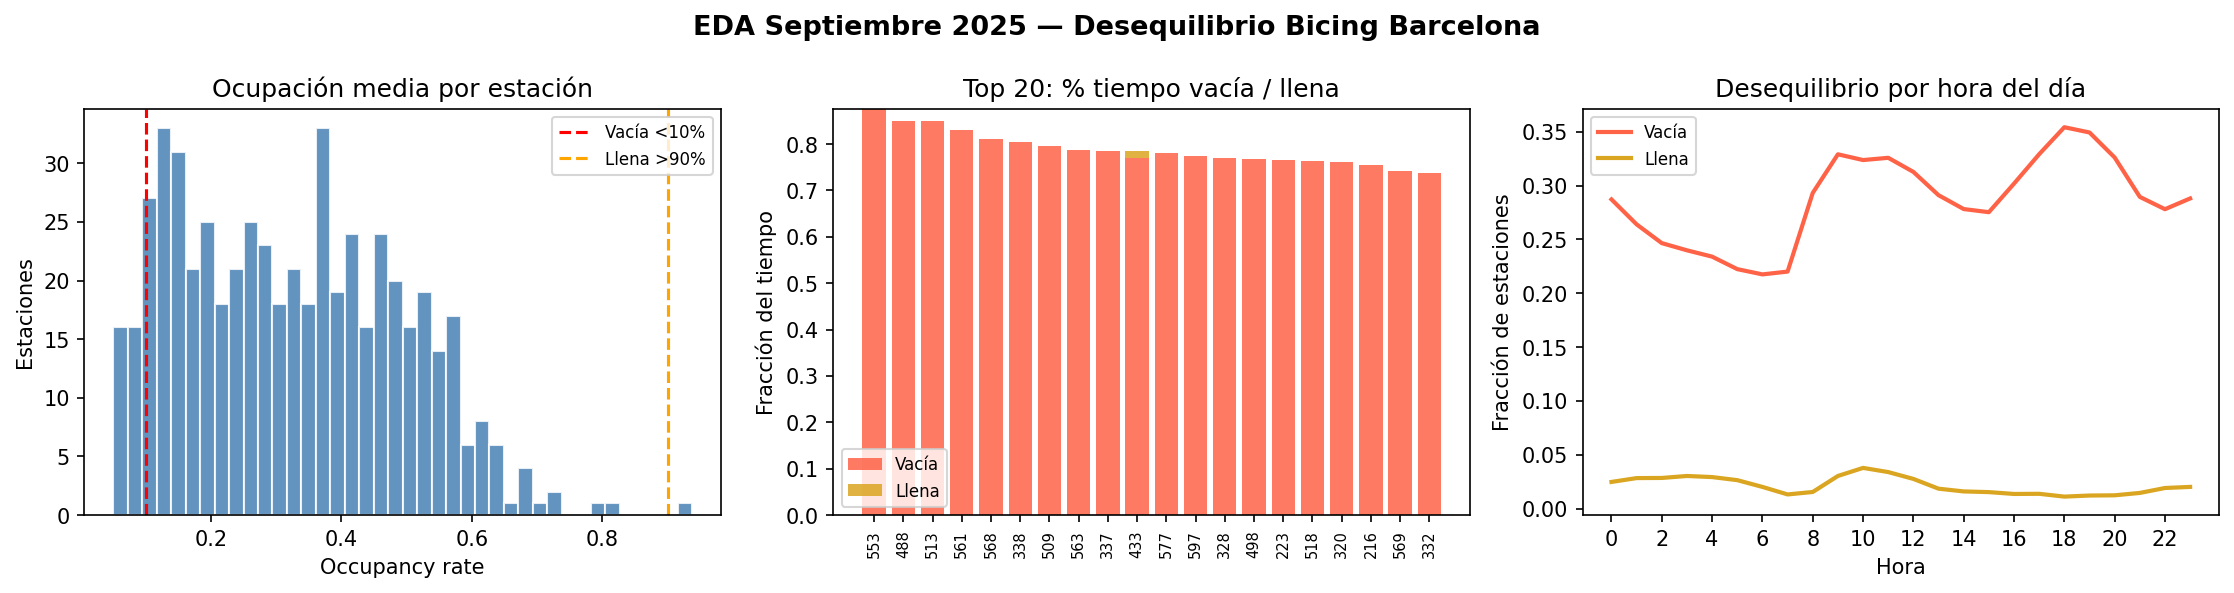
\includegraphics[width=0.9\textwidth]{BRP_01_eda_septiembre_2025__desequilibrio_bicing_barcelon.png}
\caption{Distribución de ocupación, top-20 estaciones desequilibradas y evolución
  horaria del desequilibrio en septiembre 2025. El 28,6\,\% del tiempo una estación
  cualquiera está vacía; el patrón por horas es claramente bimodal (mañana/tarde).}
\label{fig:eda_imbalance}
\end{figure}

\subsection{Efecto gravitacional de la altitud}

El EDA confirma que las estaciones situadas a mayor altitud acumulan más bicicletas
de forma sistemática (efecto gravitacional): los ciclistas suben pedalando y bajan
rodando. Esto justifica la inclusión de \texttt{altitude} como feature predictora y
tiene implicaciones directas en la planificación de rutas del BRP (las zonas altas
son fuentes naturales de superávit).

\begin{figure}[H]
\centering
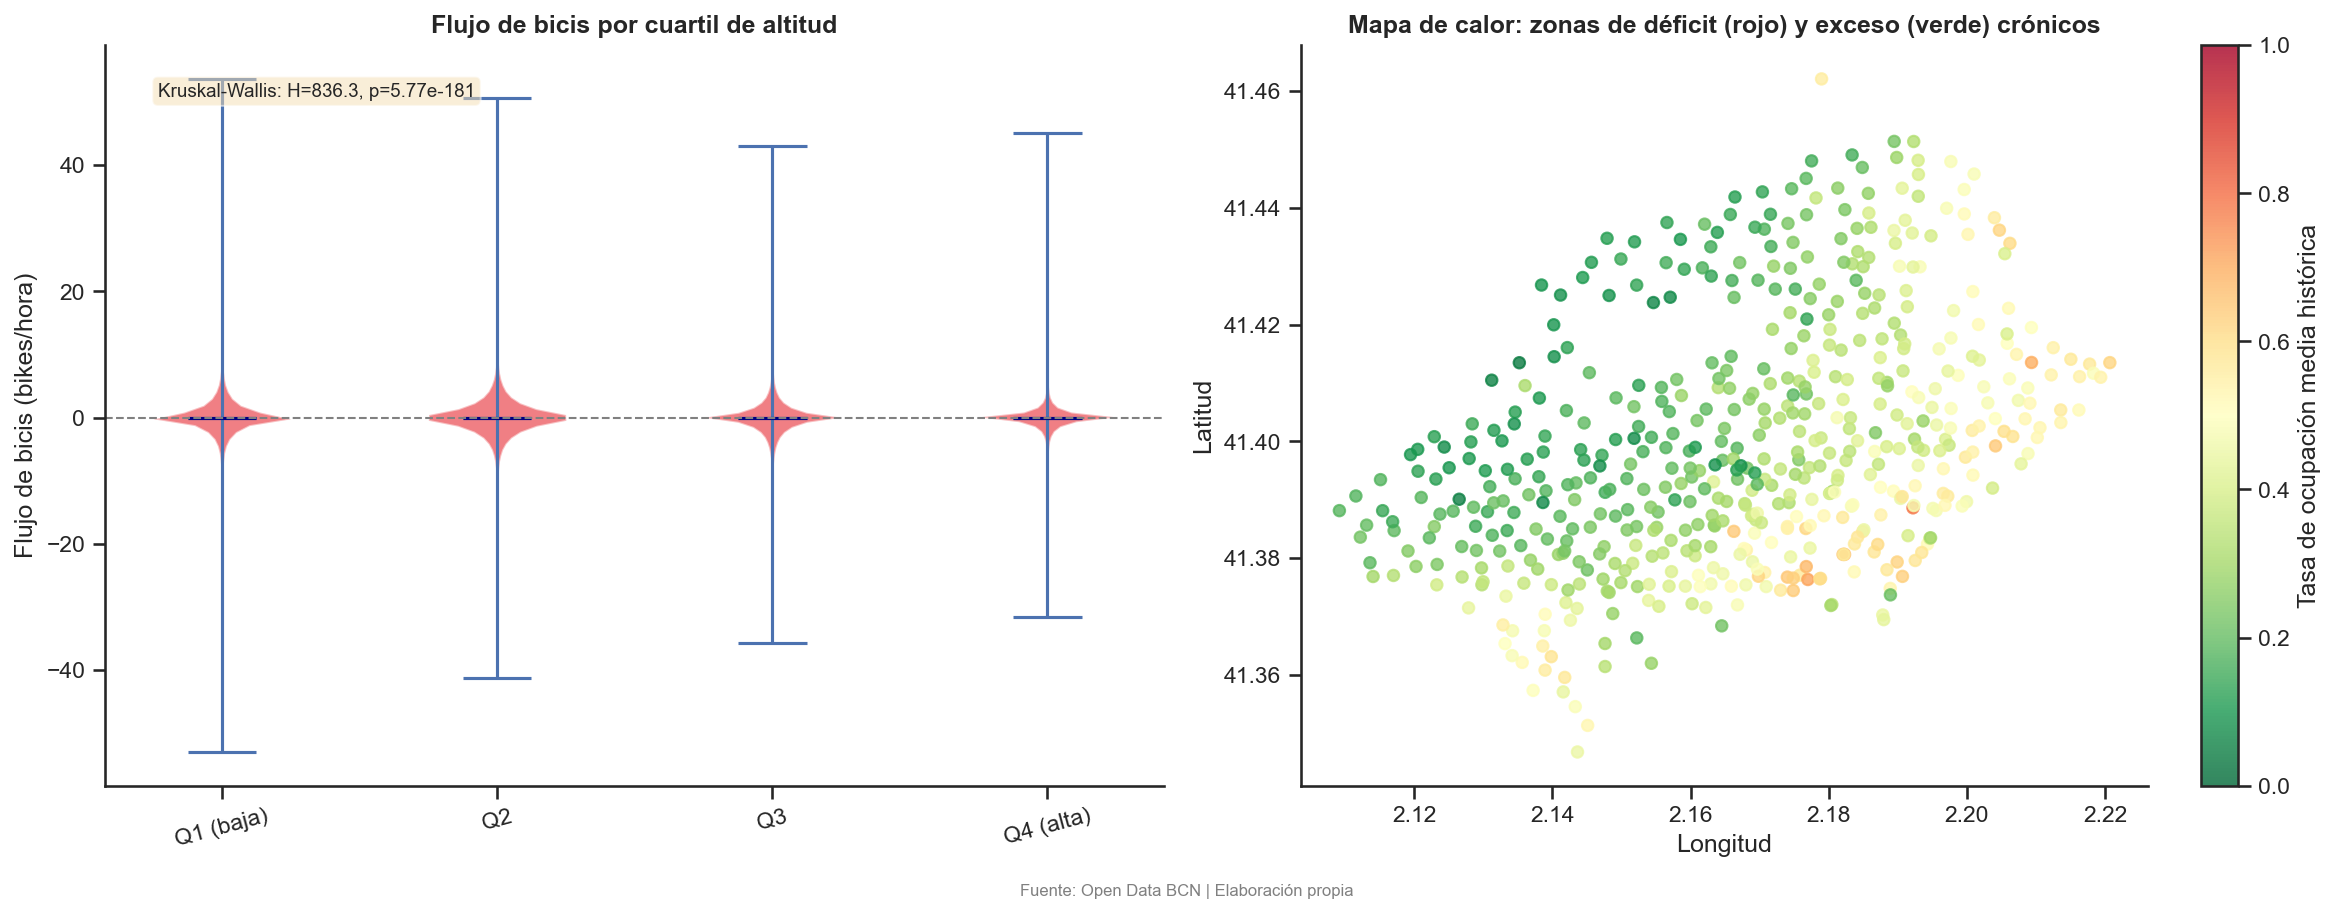
\includegraphics[width=0.75\textwidth]{EDA_12_flujo_de_bicis_por_cuartil_de_altitud.png}
\caption{Flujo neto de bicicletas por cuartil de altitud. Las estaciones en cuartiles
  superiores presentan un superávit neto sistemático.}
\label{fig:altitude_effect}
\end{figure}

% =============================================================================
\section{BRP --- Optimización de Rutas de Redistribución}
% =============================================================================

\subsection{Formulación del problema}

El BRP se formula como una variante del \textit{Vehicle Routing Problem} (VRP):

\begin{itemize}
  \item \textbf{Flota}: $K = 5$ camiones con capacidad $C = 30$ bicicletas.
  \item \textbf{Depósito}: centro logístico de Bicing (lat $= 41{,}368$, lon $= 2{,}152$)
        con reservas ilimitadas para la Fase~2.
  \item \textbf{Objetivo de ocupación}: $\tau = 50\,\%$ de la capacidad por estación.
  \item \textbf{Escenario}: martes 5 de agosto de 2025 a las 8:00\,h (primera semana
        del conjunto de test; hora punta de máximo desequilibrio).
\end{itemize}

\paragraph{Input del modelo.}
Las predicciones XGBoost reemplazan las medias históricas, convirtiendo el BRP
de \textbf{reactivo} (qué tenemos ahora) a \textbf{proactivo} (qué tendremos en 1\,h).
Para cada estación $i$:
\[
  \text{deficit}_i = \text{target}_i - \hat{y}_i \cdot \text{capacity}_i
\]
donde $\hat{y}_i$ es la predicción de \texttt{occupancy\_rate} del XGBoost.

\subsection{Algoritmo multi-fase con dispatching round-robin}

Se mejora el algoritmo greedy original con dos modificaciones clave:

\paragraph{Fase 1 -- Redistribución.}
Los camiones recogen bicicletas de estaciones con superávit y las entregan a
estaciones con déficit. La selección de parada se basa en la ratio
urgencia/distancia:
\[
  \text{score}(i) = \frac{|\text{deficit}_i|}{d(\text{pos}, i)}
\]

\paragraph{Fase 2 -- Inyección de reservas.}
Cuando se agota el superávit, los camiones vuelven al depósito para cargar bicis
de las reservas (stock del almacén Bicing) y continúan sirviendo las estaciones
más críticas. Con un presupuesto de 200 bicicletas de reserva, todos los camiones
quedan activos durante toda la operación.

\paragraph{Dispatching round-robin.}
Las decisiones se toman en turnos interleados entre camiones (no secuencialmente),
lo que distribuye el superávit de forma equitativa y evita que un camión acapare
todos los recursos. Este cambio elimina el camión inactivo del algoritmo original.

\subsection{Resultados BRP}

\begin{table}[H]
\centering
\caption{Métricas de mejora BRP (escenario mar.\ 5-ago-2025 08:00\,h).}
\label{tab:brp_results}
\begin{tabular}{lccc}
\toprule
\textbf{Métrica} & \textbf{Antes} & \textbf{Después} & $\boldsymbol{\Delta}$ \\
\midrule
Estaciones críticas      & 407 & 308 & $-24{,}3\,\%$ \\
  \quad con déficit      & 327 & 282 & $-13{,}8\,\%$ \\
  \quad con superávit    &  80 &  26 & $-67{,}5\,\%$ \\
Déficit total (bicis)    & 3.010 & 2.596 & $-13{,}8\,\%$ \\
Superávit total (bicis)  &   688 &   192 & $-72{,}1\,\%$ \\
RMSE déficit             &  8,43 &  7,26 & $-13{,}9\,\%$ \\
\midrule
Bicicletas redistribuidas (Fase~1) & \multicolumn{3}{c}{412} \\
Kilómetros totales                  & \multicolumn{3}{c}{143,5\,km} \\
Eficiencia (km/bici)                & \multicolumn{3}{c}{0,35\,km/bici} \\
\bottomrule
\end{tabular}
\end{table}

\begin{figure}[H]
\centering
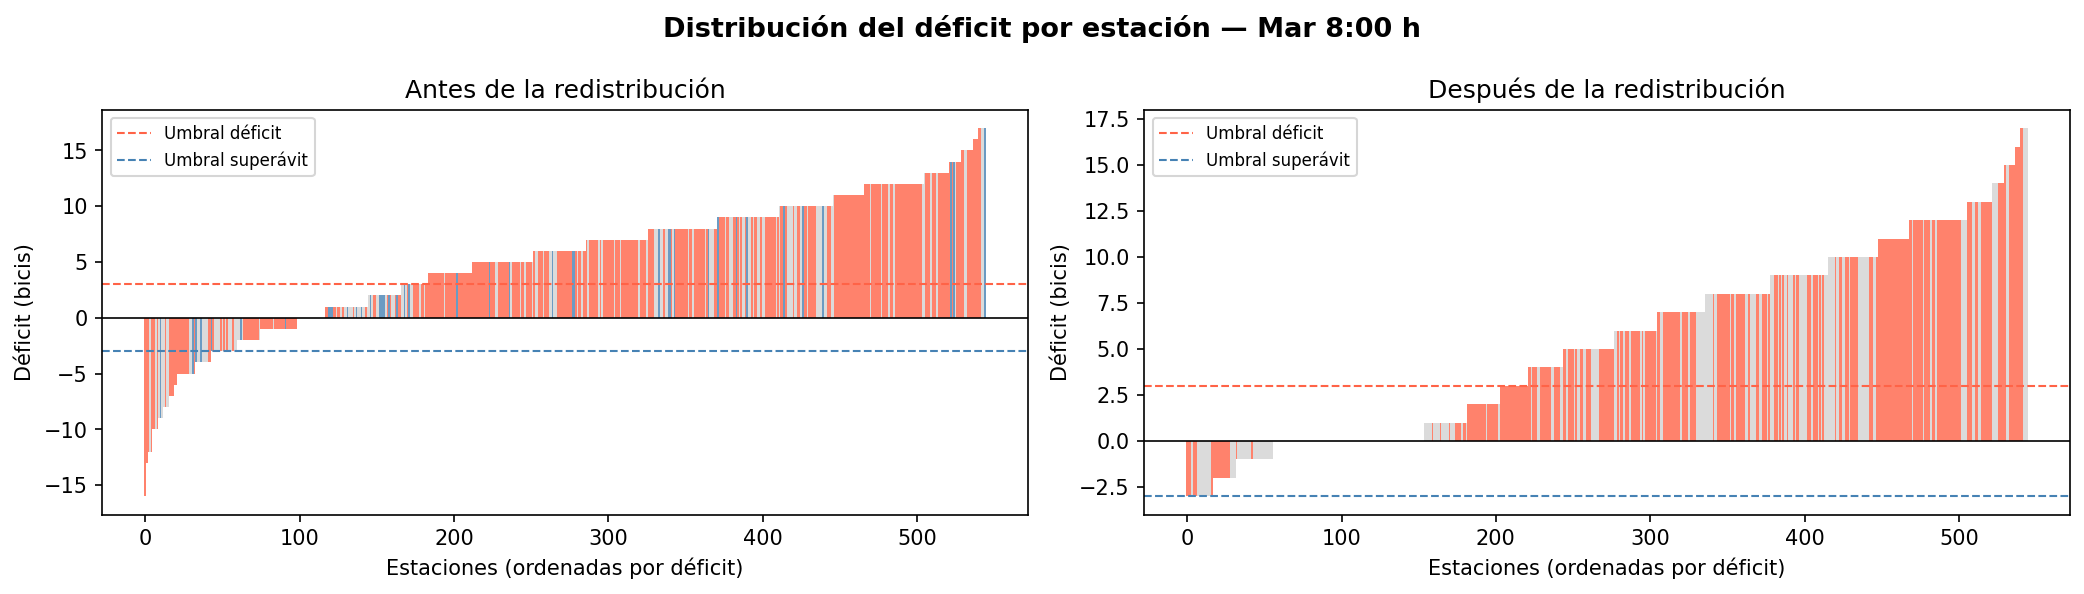
\includegraphics[width=0.85\textwidth]{BRP_04_distribución_del_déficit_por_estación__mar_800_h.png}
\caption{Distribución del déficit por estación antes y después de la redistribución.
  Las barras rojas (déficit) se reducen; las azules (superávit) desaparecen al ser
  absorbidas por los camiones.}
\label{fig:brp_deficit}
\end{figure}

\subsection{Comparación con el algoritmo original (greedy reactivo)}

\begin{table}[H]
\centering
\caption{Comparación algoritmo original vs.\ multi-fase con predicciones.}
\label{tab:brp_comparison}
\begin{tabular}{lcc}
\toprule
\textbf{Característica} & \textbf{Greedy reactivo} & \textbf{Multi-fase + modelo} \\
\midrule
Input                   & Media histórica           & Predicción XGBoost \\
Camiones activos        & 4 / 5                     & 5 / 5 \\
Selección de parada     & Vecino más cercano        & Ratio urgencia/distancia \\
Reservas del depósito   & No                        & Sí (200 bicis) \\
Despacho                & Secuencial                & Round-robin interleado \\
Horizonte temporal      & Reactivo ($t$)            & Proactivo ($t+1\,\text{h}$) \\
\bottomrule
\end{tabular}
\end{table}

% =============================================================================
\section{Conclusiones}
% =============================================================================

\subsection{Modelo predictivo}

El XGBoost con búsqueda bayesiana de hiperparámetros (Optuna, 50 trials) obtiene
el mejor rendimiento predictivo con un \textbf{MAE = 0,061} y \textbf{$R^2$ = 0,893}
en el conjunto de test, equivalente a un error medio de \textbf{1,66 bicicletas por
estación y hora}. La consistencia entre validación y test ($\Delta$MAE $= 0,001$)
descarta el sobreajuste.

El GRU simplificado, diseñado para ejecutarse en hardware modesto (Mac M1), no
alcanza rendimiento competitivo con las restricciones de lookback y épocas
aplicadas ($R^2 = 0{,}43$). Para alcanzar el potencial del modelo recurrente
serían necesarios: lookback $\geq 168\,\text{h}$, $\geq 20$ épocas y
optimización de hiperparámetros con Optuna.

\subsection{BRP}

La integración del XGBoost en el BRP convierte la planificación de rutas de
reactiva a proactiva, con las siguientes mejoras concretas:

\begin{itemize}
  \item \textbf{Predicciones en tiempo real}: el modelo anticipa el déficit con 1\,h de
        antelación, permitiendo que los camiones estén en posición antes de que
        ocurra el desequilibrio.
  \item \textbf{Todos los camiones activos}: el algoritmo round-robin garantiza que los
        5 camiones operan. En el escenario analizado se redistribuyen \textbf{412 bicicletas}
        en \textbf{143,5\,km} ($0{,}35$\,km/bici), reduciendo las estaciones críticas un
        \textbf{24,3\,\%}.
  \item \textbf{Priorización por urgencia}: la ratio urgencia/distancia reduce los
        kilómetros por bicicleta redistribuida respecto al vecino más cercano puro.
\end{itemize}

\subsection{Limitaciones y trabajo futuro}

\paragraph{Modelo.}
\begin{itemize}
  \item Sin información de redistribuciones pasadas: el modelo no sabe si una estación
        acaba de ser reabastecida (genera errores escalón).
  \item Sin features de red: la interdependencia entre estaciones vecinas no está capturada.
  \item El GRU requiere más recursos computacionales para competir con XGBoost.
\end{itemize}

\paragraph{BRP.}
\begin{itemize}
  \item La heurística greedy no garantiza la solución óptima global.
  \item Distancias euclídeas (Haversine): sin tráfico, semáforos ni topografía viaria.
  \item Escenario estático: se asume que las bicicletas no se mueven durante la
        operación de redistribución.
  \item Posibles mejoras: metaheurísticas (Simulated Annealing, ALNS), enrutamiento
        con OSRM, predicción de múltiples horizontes temporales.
\end{itemize}

\subsection{Conclusión operativa}

El pipeline completo --- EDA $\to$ XGBoost $\to$ BRP multi-fase --- es reproducible,
modular y deployable. Con un error medio de $\sim$1,7 bicicletas por estación, el
sistema puede priorizar intervenciones en estaciones con ocupación predicha fuera
de la banda $[10\,\%, 90\,\%]$ con suficiente precisión para guiar decisiones
operativas. El artefacto \texttt{xgboost\_bicing.ubj} está listo para integración
en un sistema de soporte a la decisión en producción.

% =============================================================================
\appendix
\section{Apéndice: Estructura del repositorio}
% =============================================================================

\begin{lstlisting}
brp_bicing/
|-- notebooks/
|   |-- EDA.ipynb          # Analisis exploratorio y feature engineering
|   |-- XGBoost.ipynb      # Modelo XGBoost
|   |-- LSTM.ipynb         # Modelo GRU
|   +-- BRP.ipynb          # Optimizacion de rutas
|-- data/
|   |-- raw/               # Datos crudos de la API Bicing
|   |-- processed/         # Parquets procesados
|   +-- output/            # Figuras generadas
|-- models/
|   |-- xgboost_bicing.ubj # Modelo XGBoost serializado
|   +-- lstm_bicing.keras  # Modelo GRU serializado
+-- informe/
    +-- informe_brp_bicing.tex
\end{lstlisting}

\end{document}
